\documentclass[twoside, 12pt]{article}

\usepackage[sc]{mathpazo} % Use the Palatino font
\usepackage[T1]{fontenc} % Use 8-bit encoding that has 256 glyphs
\linespread{1.5} % Line spacing - Palatino needs more space between lines

%\usepackage[twoside,width=16cm,height=24cm,left=3cm]{geometry}
\usepackage[hmarginratio=1:1,top=20mm,width=20cm,height=23.7cm,columnsep=15pt]{geometry} % Document margins
\usepackage{multicol} % Used for the two-column layout of the document
\usepackage[hang, small,labelfont=bf,up,textfont=it,up]{caption} % Custom captions under/above floats in tables or figures
\usepackage{booktabs} % Horizontal rules in tables
\usepackage{float} % Required for tables and figures in the multi-column environment - they need to be placed in specific locations with the [H] (e.g. \begin{table}[H])
\usepackage{hyperref} % For hyperlinks in the PDF

%----------- Agregados para el caso de ustedes -------------------------------
\usepackage[spanish]{babel}% idioma castellano
\usepackage[utf8]{inputenc}% esto es para poder poner los tildes directamente. Puede que cambie de versión a versión de sistema operativos (más información en http://www.aq.upm.es/Departamentos/Fisica/agmartin/webpublico/latex/FAQ-CervanTeX/FAQ-CervanTeX-6.html )
\usepackage{graphicx} % para insertar figuras
\usepackage{subfigure} % para insertar figuras dentro de figuras
\usepackage{times} % plataforma
\usepackage{amsmath} % --para ecuaciones y algunos símbolos 
\usepackage{wrapfig,lipsum}
\usepackage{listings}
\usepackage{color}

\definecolor{dkgreen}{rgb}{0,0.6,0}
\definecolor{gray}{rgb}{0.5,0.5,0.5}
\definecolor{mauve}{rgb}{0.58,0,0.82}

\lstset{frame=tb,
	language=C++,
	aboveskip=3mm,
	belowskip=3mm,
	showstringspaces=false,
	columns=flexible,
	basicstyle={\small\ttfamily},
	numbers=none,
	numberstyle=\tiny\color{gray},
	keywordstyle=\color{blue},
	commentstyle=\color{dkgreen},
	stringstyle=\color{mauve},
	breaklines=true,
	breakatwhitespace=true,
	tabsize=3
}
% ---------------------- -----------------------------------------------------

\usepackage{lettrine} % The lettrine is the first enlarged letter at the beginning of the text
\usepackage{paralist} % Used for the compactitem environment which makes bullet points with less space between them
\usepackage[T1]{fontenc}					%para poder usar tildes sin problemas

\usepackage{mathrsfs}
% Abreviaturas
%\newcommand\RR{\mathbb{R}}

\providecommand{\dpart}[2]{\frac{\partial#1}{\partial#2}}

\graphicspath{{Imagenes/}}

\begin{document}
	
\begin{center}
	{\fontsize{20pt}{10pt}\textbf{Choque unidimensional bajo potencial de Pauli}}
\end{center}

\section{Implementación de Pauli}

\subsection{Características generales}

El potencial de Pauli, debido a su dependencia en el momento, no es candidato para heredar las propiedades de un potencial \texttt{ShortRange} como Morse o Lennard-Jones

\[ V_{P}(q,p) = D\sum_{i<j} e^{-\frac{1}{2}s_{ij}^2} \qquad \text{;} \qquad s_{ij}^2 = \frac{|\mathbf{p}_i - \mathbf{p}_j|^2}{p_o^2} + \frac{|\mathbf{q}_i - \mathbf{q}_j|^2}{q_o^2}\]

Un Hamiltoneano interactuando con un potencial dependiente de momentos tendrá ecuaciones

\begin{align*}
\dot{\mathbf{q}}_i &= \dpart{H}{\mathbf{p}_i} = \frac{\mathbf{p}_i}{m} + \dpart{V_P}{\mathbf{p}_i} \equiv \frac{\mathbf{p}_i}{m} - \sum_{j\neq i} \mathbf{G}_{ij} \\ 
\dot{\mathbf{p}}_i &= -\dpart{H}{\mathbf{q}_i} = -\dpart{V_P}{\mathbf{p}_i} \equiv \sum_{j\neq i} \mathbf{F}_{ij}
\end{align*}

donde definimos las \textit{guerzas} $\mathbf{G}$ análogamente a las fuerzas habituales $\mathbf{F}$. 

Para el potencial de Pauli, las guerzas cumplen $\mathbf{G}_{ij} = -\mathbf{G}_{ji}$ al igual que las fuerzas dado que $V_P$ depende de $\mathbf{p}_i - \mathbf{p}_j$. Además, para este potencial toman la forma

\begin{align*}
\sum_{j\neq i} \mathbf{F}_{ij} &= -D \sum_{i<j} \left(-\frac{1}{2}\right)\dpart{s_{ij}^2}{\mathbf{q}_i}e^{-\frac{1}{2}s_{ij}^2} = D \sum_{i\neq j} \frac{\mathbf{q}_i - \mathbf{q}_j}{q_o^2}e^{-\frac{1}{2}s_{ij}^2} \Longrightarrow \mathbf{F}_{ij} = (\mathbf{q}_i - \mathbf{q}_j)\frac{D}{q_o^2}e^{-\frac{1}{2}s_{ij}^2} \\
\sum_{j\neq i} \mathbf{G}_{ij} &= -D \sum_{i<j} \left(-\frac{1}{2}\right)\dpart{s_{ij}^2}{\mathbf{p}_i}e^{-\frac{1}{2}s_{ij}^2} = D \sum_{i\neq j} \frac{\mathbf{p}_i - \mathbf{p}_j}{p_o^2}e^{-\frac{1}{2}s_{ij}^2} \Longrightarrow \mathbf{G}_{ij} = (\mathbf{p}_i - \mathbf{p}_j)\frac{D}{p_o^2}e^{-\frac{1}{2}s_{ij}^2}
\end{align*}

Según lo esperado, dada la simetría entre $p$ y $q$ en $V_P$, las expresiones resultan completamente análogas. 

\subsection{Pauli class}

A pesar de no heredar de \texttt{ShortRange}, resulta natural pensar que este potencial tendrá un radio de corte en el espacio de fases $s_{cut}$ con su $shift\_style$ correspondiente. Además, tendrá los parámetros 
esperados $q_o$, $p_o$ y $D$.

Esta clase compartirá con \texttt{ShortRange} las funciones \texttt{pair\_force}, \texttt{pair\_energ} y \texttt{forces}. Además, tendrá que tener sus equivalentes para las guerzas \texttt{pair\_gorce} y \texttt{gorces}. 
Utilizando la misma filosofía que en la implementación de Morse anterior, implementamos en \texttt{C} las contrapartes de estas funciones según 

\begin{multicols}{2}
\begin{lstlisting}
float forces(...){
	...
	for(i=0;i<N;i++){
		for(j=i+1;j<N;j++){
			pair_force(...)
			pair_energ(...)
		}	
		...
	}
	...
}


float gorces(...){
	...
	for(i=0;i<N;i++){
		for(j=i+1;j<N;j++){
			pair_gorce(...)
			pair_energ(...)
		}	
		...
	}
...
}

\end{lstlisting} 
\columnbreak
\begin{lstlisting}
float pair_force(..){
	...
	calculo de 
	parametros
	...
}



float pair_gorce(..){
	...
	calculo de 
	parametros
	...
}



float pair_energ(..){
	...
	calculo de 
	parametros
	...
}

\end{lstlisting} 
\end{multicols}

Esta implementación por separado del cálculo de fuerzas y guerzas resulta apropiado teniendo en mente los \textit{splitting methods} a la hora de integrar, donde se integra $q$ y $p$ por separado y, por lo tanto, 
no necesariamente se calculan las fuerzas y las guerzas simultáneamente.

Sin embargo, para integradores que si calculan fuerzas y guerzas simultáneamente, resulta natural explotar la simetría a la hora de calcular $\mathbf{F}_{ij}$ y $\mathbf{G}_{ij}$, calculando el término 
$e^{-\frac{1}{2}s_{ij}^2}$ una única vez. Por lo tanto, implementamos una sexta función combinada \texttt{fgorces} en \texttt{Python} con su contraparte en \texttt{C}.

Para comparar rapidamente ambas implementaciones, corrimos 10000 las funciones \texttt{forces} y \texttt{gorces} para $N_{part} = 1000$ y registramos el tiempo. 
Lo mismo hicimos para \texttt{fgorces}, asegurándonos de que los resultados fuesen los mismos. 
Obtuvimos entonces que la versión separada tardaba $\sim 65\%$ más que la combinada, bastante razonable si pensamos que la exponencial es la parte más costosa del cómputo y estamos calculándola la mitad de las veces.

\section{Estudio de integradores}

\subsection{Integradores implementados}

Dado que el Hamiltoneano es no separable, no encontramos integradores simplécticos y explícitos. 
Con el objetivo de comparar, decidimos implementar 2 integradores no simplécticos pero explícitos y un integrador simpléctico pero no explícito. 

\subsection{Conservación de la energía}

qi = 6
pi =-4
D = 10000
qo = 1 = po
h = 0.01

\begin{figure}[h]
	\centering
	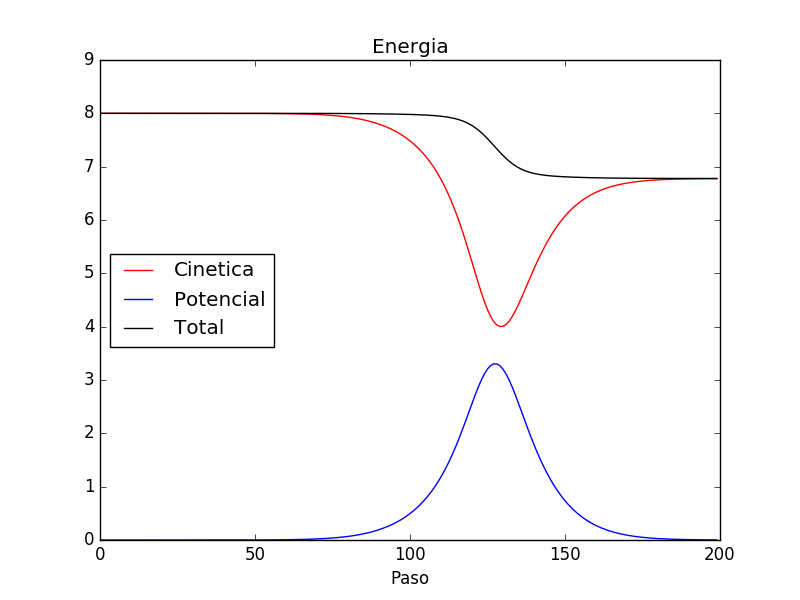
\includegraphics[trim = 20mm 0mm 15mm 10mm, clip, width=0.32\columnwidth]{energia_euler_0,01.png}
	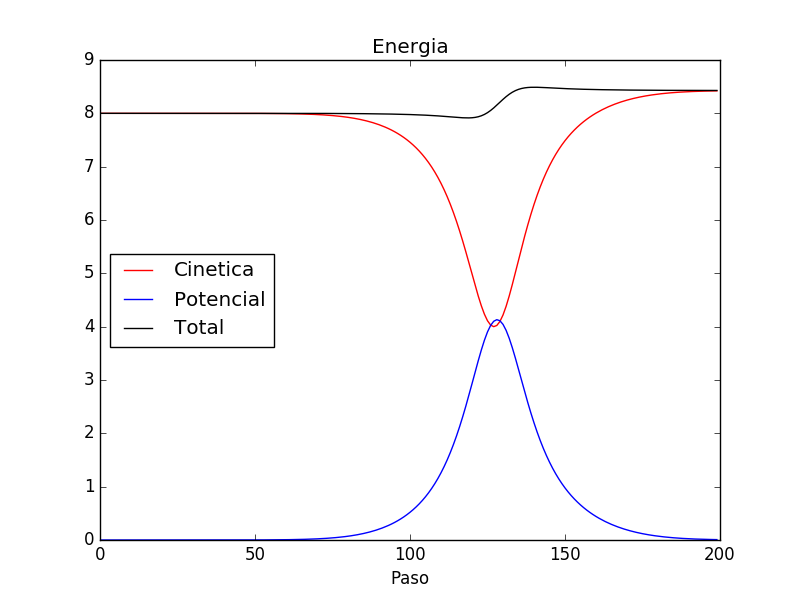
\includegraphics[trim = 20mm 0mm 15mm 10mm, clip, width=0.32\columnwidth]{energia_rk2_0,01.png}
	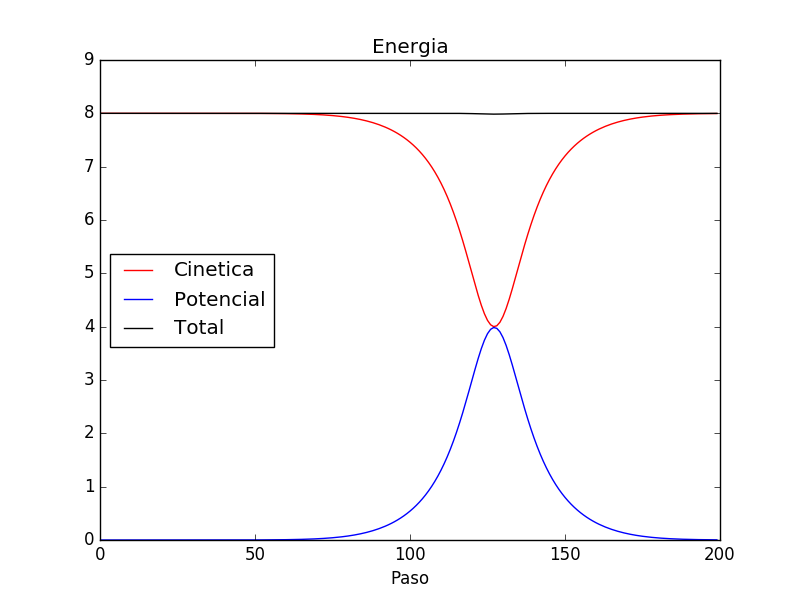
\includegraphics[trim = 20mm 0mm 15mm 10mm, clip, width=0.32\columnwidth]{energia_mpr_0,01.png}
	\caption{}
	\label{fig:histogramas}
\end{figure}


\subsection{Espacio de fases}



\section{Conclusiones}

\end{document}